%%%%%%%%%%%%%%%%%%%%%%%%%%%%%%%%%%%%%%%%%%%%%%%%%%%%%%%%%%%%%%
%% Carlos Segarra's Beamer Presentation Template. All credits
%% to Vincent Labatut from whom I took the template and added
%% my own flavour to it. Kudos to <vincent.labatut@univ-avignon.fr>
%%%%%%%%%%%%%%%%%%%%%%%%%%%%%%%%%%%%%%%%%%%%%%%%%%%%%%%%%%%%%%
% setup Beamer
\documentclass[10pt,    % default is 11pt, use 10pt for more compact slides
%    handout,            % collapse all overlays (=animations) and video-invert console text
    english,            % presentation language (theme supports only french & english)
    xcolor=table,       % colors in the tables
    envcountsect,        % include section number in theorem numbers
    aspectratio=169     % Using 16:9 aspect ratio because 2019
]{beamer}

%%%%%%%%%%%%%%%%%%%%%%%%%%%%%%%%%%%%%%%%%%%%%%%%%%%%%%%%%%%%%%
% setup the theme
%\usepackage{au/sty/beamerthemeAU}         % no option at all
\usepackage[light]{csg-temp/sty/beamerthemeAU}   % the "light" option only changes the title and section pages

%%%%%%%%%%%%%%%%%%%%%%%%%%%%%%%%%%%%%%%%%%%%%%%%%%%%%%%%%%%%%%
% setup side notes
\usepackage{pgfpages}                                   % comment all 3 below lines to hide notes
%\setbeameroption{show notes}                           % alternate content and note slides
%\setbeameroption{show only notes}                      % only note slides
%\setbeameroption{show notes on second screen=right}    % dualscreen: right, left, top, bottom
%\usepackage{enumitem}

%%%%%%%%%%%%%%%%%%%%%%%%%%%%%%%%%%%%%%%%%%%%%%%%%%%%%%%%%%%%%%
% name of the biblatex file
\addbibresource{biblio.bib}

%%%%%%%%%%%%%%%%%%%%%%%%%%%%%%%%%%%%%%%%%%%%%%%%%%%%%%%%%%%%%%
% External Packages
\usepackage{datenumber}
\usepackage{varwidth}

% Math Mode
%\usepackage{algorithm}
%\usepackage{algorithmic}
%\usepackage{algorithm2e}
%\usepackage{multicol}
%\usepackage[noend]{algpseudocode}

%%%%%%%%%%%%%%%%%%%%%%%%%%%%%%%%%%%%%%%%%%%%%%%%%%%%%%%%%%%%%%
% title and subtitle of the presentation (the latter is optional)
\newcommand{\mainTitle}{Checkpoint Restore of Container Meshes}
\newcommand{\secondTitle}{Design, Implementation, and Evaluation}
\subtitle{Decentralized Systems - Project Proposal} % leave empty if no subtitle
\title[\mainTitle] % leave empty for no title in footer
    {\Large \mainTitle \\ \normalsize \secondTitle}
\subtitle{Decentralized Systems - Project Proposal} % leave empty if no subtitle
%\subtitle{Master in Research in Informatics - MIRI}
%%%%%%%%%%%%%%%%%%%%%%%%%%%%%%%%%%%%%%%%%%%%%%%%%%%%%%%%%%%%%%
% date of the presentation (leave empty for no date, default is today)
\date[March 13, 2020] % leave empty for no date in footer
    {Friday March 13, 2020}
    %{\datedayname, \today}
%%%%%%%%%%%%%%%%%%%%%%%%%%%%%%%%%%%%%%%%%%%%%%%%%%%%%%%%%%%%%%
% authors and their affiliations (the latter is optional)
\author[] % leave empty for no author in footer
{Carlos Segarra - \texttt{carlos.segarra@estudiant.upc.edu}}
%{\inst{1} Computer Science Lab, Avignon University -- LIA EA 4128 \texttt{\{firstname.lastname\}@univ-avignon.fr}
%\and \inst{2} Institute of Disruptive Innovation, University of Excellence \texttt{\{firstname.lastname\}@univ-excell.fr}
%}
%%%%%%%%%%%%%%%%%%%%%%%%%%%%%%%%%%%%%%%%%%%%%%%%%%%%%%%%%%%%%%
% optional: additional logo (ex. lab)
%\titlegraphic{
\includegraphics[width=3cm,]{images/logo_FME.png}}
% if you want several logos, put them in a box
%\titlegraphic{\parbox{3cm}{\includegraphics[width=3cm,]{images/ceri_logo.pdf}\newline\includegraphics[width=3cm,]{images/lia_logo.pdf}}}
%%%%%%%%%%%%%%%%%%%%%%%%%%%%%%%%%%%%%%%%%%%%%%%%%%%%%%%%%%%%%%

%%%%%%%%%%%%%%%%%%%%%%%%%%%%%%%%%%%%%%%%%%%%%%%%%%%%%%%%%%%%%
% Presentation speciphic packages
% \usepackage{multicol}
% \usepackage[titles]{tocloft}
% \renewcommand{\cftchapfont}{\normalfont\bfseries}
\usetikzlibrary{decorations.pathmorphing, patterns}
\usepackage{tabularx}
\newcolumntype{L}[1]{>{\raggedright\arraybackslash}p{#1}}
\newcolumntype{C}[1]{>{\centering\arraybackslash}p{#1}}
\newcolumntype{R}[1]{>{\raggedleft\arraybackslash}p{#1}}
%%%%%%%%%%%%%%%%%%%%%%%%%%%%%%%%%%%%%%%%%%%%%%%%%%%%%%%%%%%%%

%%%%%%%%%%%%%%%%%%%%%%%%%%%%%%%%%%%%%%%%%%%%%%%%%%%%%%%%%%%%%%
\begin{document}
%%% title page
\begin{frame}
  \titlepage
\end{frame}

\begin{frame}
    \frametitle{Problem Statement and Motivation}
    \framesubtitle{Outline of the Project}

    \vspace{-25pt}

    \textbf{\textcolor{blue}{Problem Motivation:}}
    \begin{itemize}
        \small
        \item Containers have become the go-to alternative for sandboxing and deploying several distributed applications. 
        \item Orchestrators such as \href{https://kubernetes.io/}{Kubernetes} or \href{https://docs.docker.com/engine/swarm/}{Docker Swarm} ease these deployments and the network configuration, making it transparent to the user.
        \item \href{https://en.wikipedia.org/wiki/Application_checkpointing}{Checkpointing} provides systems with fault-tolerance and state consistency enabling rollback and restore from previous stable versions.
            Live migration consists in transparently relocating running services for improved resource-management or increased QoS.
        \item Support for checkpointing (Docker) containers is very limited (\href{https://github.com/docker/cli/blob/master/experimental/checkpoint-restore.md}{[1]}, \href{https://criu.org/Docker}{[2]}) and only in experimental mode. 
    \end{itemize}

    \small
    \begin{alertblock}{Main Goal}
        Design, implementation, and evaluation of a distributed checkpoint/restore algorithm for a container mesh.
    \end{alertblock}

\end{frame}

\begin{frame}
    \frametitle{TL-DR}
    \framesubtitle{Outline of the Project}

    \begin{columns}
        \begin{column}{.55\textwidth}
            \textbf{Tracker-Based Bittorrent Protocol:}
            \begin{itemize}
                \item \textbf{Bittorrent} is a peer-to-peer communication protocol for file sharing.
                \item A \textbf{Bittorrent} tracker is a server that assists in the communication between peers.
                \item It keeps track of where file copies reside.
            \end{itemize}
            \textbf{The ALTO Service Architecture:}
            \begin{itemize}
                \item The \textbf{\href{https://tools.ietf.org/html/rfc7285}{Application Layer Traffic Optimization}} services provide network information with the goal of modifying network resources consumption.
            \end{itemize}
        \end{column}
        \hfill
        \begin{column}{.35\textwidth}
            \begin{figure}[h!]
                \centering
                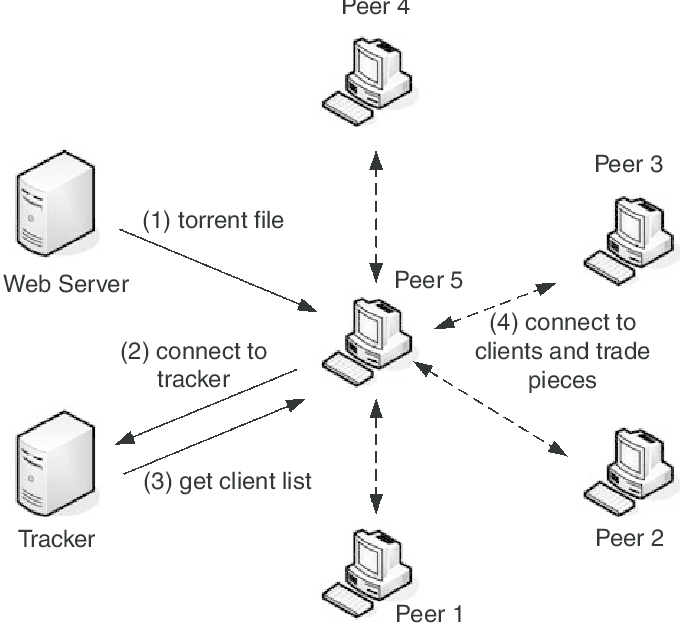
\includegraphics[width=\textwidth]{./images/bit-torrent.png}
                \caption{Bittorrent Tracker Protocol Architecture}
            \end{figure}
        \end{column}
    \end{columns}

\end{frame}

\begin{frame}
    \frametitle{Proposed Architecture}

    \vspace{-15pt}
    \begin{columns}
        \begin{column}{.35\textwidth}
            \textbf{Exectuion Flow:}
            \begin{enumerate}
                \item Peer node queries tracker for list of peers.
                \item Tracker forwards request to ALTO Server.
                \item Server delegates to respective WMN Agent.
                \item Server aggregates responses and returns sorted list to Tracker.
                \item Tracker forwards response to asking peer.
            \end{enumerate}
        \end{column}
        \begin{column}{.70\textwidth}
            \begin{figure}[h!]
                \centering
                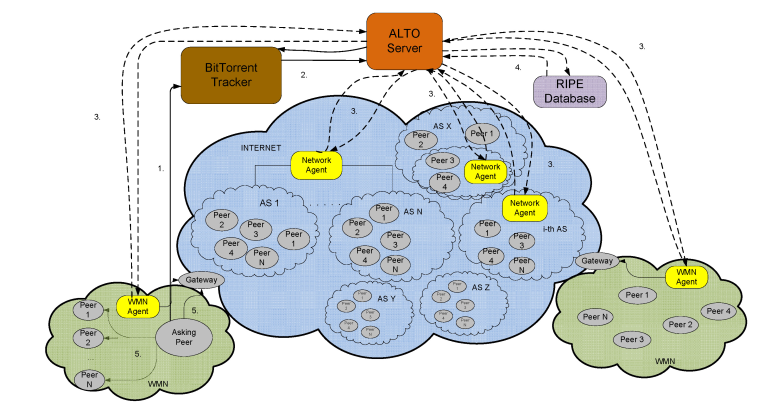
\includegraphics[width=1.05\textwidth]{./images/architecture.png}
            \end{figure}
        \end{column}
    \end{columns}

\end{frame}

\begin{frame}
    \frametitle{Open Questions}

    \begin{enumerate}
        \item What's your opinion about the evaluation section?
        \begin{itemize}
            \item What experiments do they lay out?
            \item What do they show?
            \item What does that prove?
            \item What is the statistical relevance of the results?
            \item Who they compare against?
        \end{itemize}
        \item Are Tracker-Based Bittorent Protocols used anymore?
        \item What's your opinion on the design choice for the ALTO Server?
    \end{enumerate}

\end{frame}



\end{document}
